\documentclass[11pt,a4paper]{article}

\usepackage[margin=0.9in]{geometry}
\usepackage{graphicx}
\usepackage{pdfpages}
\usepackage{booktabs}
\usepackage{float}
\usepackage{natbib}
\usepackage{newtxtext,newtxmath}
\usepackage[hidelinks]{hyperref}

\graphicspath{{./}}
\emergencystretch=2em

\title{Kramer spherical Stokes benchmark}
\author{}
\date{}

\begin{document}

\maketitle
\vspace{-2.0em}

\section{Introduction}

The Kramer spherical benchmark verifies incompressible Stokes flow in a three-dimensional spherical shell using analytical solutions derived by \citet{kramer2021}. Such tests are essential for mantle-convection codes, where curved geometry, free-slip boundaries, spherical harmonic forcing, and stress recovery all affect the accuracy of geodynamic observables. The benchmark is particularly useful because it includes both smooth volumetric forcing and delta-function forcing on an internal spherical interface, together with free-slip and zero-slip boundary conditions. It therefore tests not only velocity and pressure convergence, but also the robustness of boundary-condition enforcement and stress post-processing in spherical geometry.

\section{Governing equations and benchmark setup}

The model solves the incompressible Stokes equations
\[
  -\nabla \cdot \boldsymbol{\sigma} = \rho \mathbf{g},
  \qquad
  \nabla \cdot \mathbf{u}=0,
\]
with constant viscosity and spherical-shell radii \(R_-=1.22\) and \(R_+=2.22\). Delta-function cases use an internal interface at \(R_{\mathrm{int}}=2.0=(R_-+R_+)/2\). Smooth cases prescribe \(\rho=(r/R_+)^kY_l^m\), while delta cases prescribe forcing proportional to \(\delta(r-R_{\mathrm{int}})Y_l^m\). The smooth cases use \(k=l+1\), following \citet{kramer2021}.

The Underworld3 calculations use a \(P_2\)--\(P_1\) Taylor--Hood discretisation with quadratic velocity and linear pressure on tetrahedral spherical-shell meshes. The reported resolutions are \(h=1/8,1/16,1/32,\) and \(1/64\). Free-slip conditions are imposed weakly, while zero-slip cases use essential velocity constraints. Solver tolerances were chosen so that discretisation error dominates the reported convergence rates. Curved-shell geometry is represented by the spherical mesh used in the benchmark output.

\begin{table}[H]
\centering
\caption{Kramer spherical benchmark cases used in the UW3 verification runs.}
\label{tab:kramer_cases}
\begin{tabular}{cllll}
\toprule
Case & Forcing & Boundary condition & \((l,m,k)\) values & Resolutions \\
\midrule
1 & delta-function & free-slip & \((2,1,3),(4,2,5),(8,4,9)\) & \(1/8\)--\(1/64\) \\
2 & smooth & free-slip & \((2,1,3),(4,2,5),(8,4,9)\) & \(1/8\)--\(1/64\) \\
3 & delta-function & zero-slip & \((2,1,3),(4,2,5),(8,4,9)\) & \(1/8\)--\(1/64\) \\
4 & smooth & zero-slip & \((2,1,3),(4,2,5),(8,4,9)\) & \(1/8\)--\(1/64\) \\
\bottomrule
\end{tabular}
\end{table}

\section{Analytical fields}

\begin{figure}[H]
    \centering
    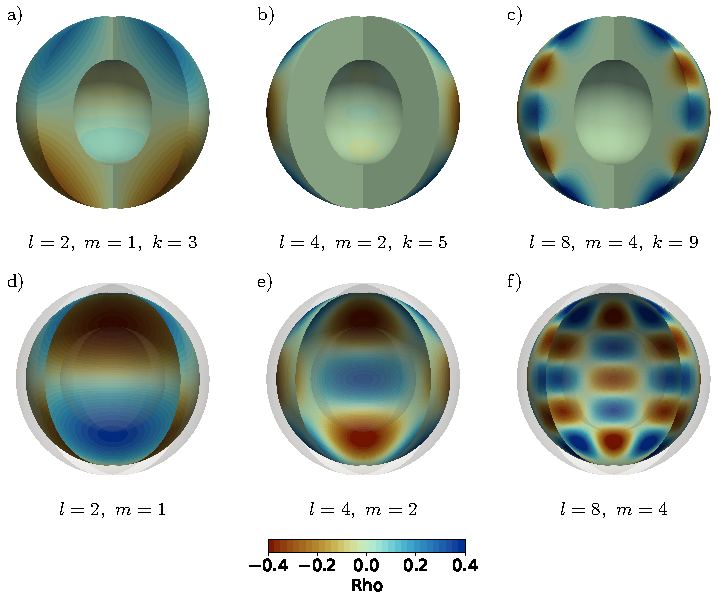
\includegraphics[width=0.98\linewidth]{figure_2_kramer_rho_ana.pdf}
    \caption{Analytical density fields. The upper row shows smooth forcing and the lower row shows delta-function forcing on \(R_{\mathrm{int}}=2.0\). Columns correspond to \((l,m,k)=(2,1,3)\), \((4,2,5)\), and \((8,4,9)\).}
    \label{fig:kramer_density_fields}
\end{figure}

Figure~\ref{fig:kramer_density_fields} illustrates the imposed density fields. Increasing \(l\) and \(m\) increases angular complexity and gives smaller-scale spherical harmonic structure. In the smooth cases, increasing \(k\) concentrates the forcing radially toward the outer boundary. In the delta cases, the forcing is localised on the internal interface, making the solution less regular than in the smooth cases.

\section{Numerical results}

\subsection{Velocity convergence}

Velocity errors are measured using relative volume \(L_2\) norms. For sufficiently smooth solutions and accurately represented curved geometry, a \(P_2\) velocity field can exhibit third-order \(L_2\) convergence \citep{girault1986,boffi2013}. The UW3 smooth spherical cases do not reach this ideal rate over the tested resolutions. Case~2 (smooth, free-slip) gives velocity rates mostly between 1.9 and 2.1, and Case~4 (smooth, zero-slip) is similarly close to second order, with some higher pre-asymptotic rates on coarser refinements. This indicates that the smooth velocity error is currently limited by curved-geometry representation, boundary-condition enforcement, mesh resolution, or a combination of these effects, rather than by the polynomial approximation alone. The result should therefore be interpreted as robust convergence, but not yet the full asymptotic \(P_2\) velocity rate reported by \citet{kramer2021} for their curved/isoparametric Fluidity setup.

For delta-function forcing, Cases~1 and 3 show reduced velocity convergence. The finest-grid rates are close to \(O(h^{1.5})\), with the zero-slip case slightly lower for some high-order spherical harmonics. This behaviour is consistent with \citet{kramer2021}. The singular forcing at \(R_{\mathrm{int}}\) reduces solution regularity, so the finite-element velocity error is not expected to follow the smooth-solution rate even when the internal interface is geometrically represented.

\subsection{Pressure convergence}

Pressure errors are also measured using relative volume \(L_2\) norms. For smooth forcing, the \(P_1\) pressure field is expected to converge at second order, and the UW3 results are consistent with this expectation: both smooth free-slip and smooth zero-slip cases give pressure rates very close to \(O(h^2)\) across the tested spherical harmonics. This agreement indicates that pressure normalisation, the Stokes solve, and the smooth analytical forcing are implemented consistently.

The delta-function cases show substantially reduced pressure convergence, approximately \(O(h^{0.5})\), in agreement with \citet{kramer2021}. This behaviour is not a solver failure; it reflects the limited regularity of the pressure solution and the difficulty of representing an interface-localised forcing with a continuous pressure discretisation. Kramer et al. specifically discuss this continuous-pressure limitation for delta-function cases. The reduced pressure rate is therefore expected, especially near the internal interface and in boundary-sensitive diagnostics where pressure enters directly.

\begin{figure}[H]
    \centering
    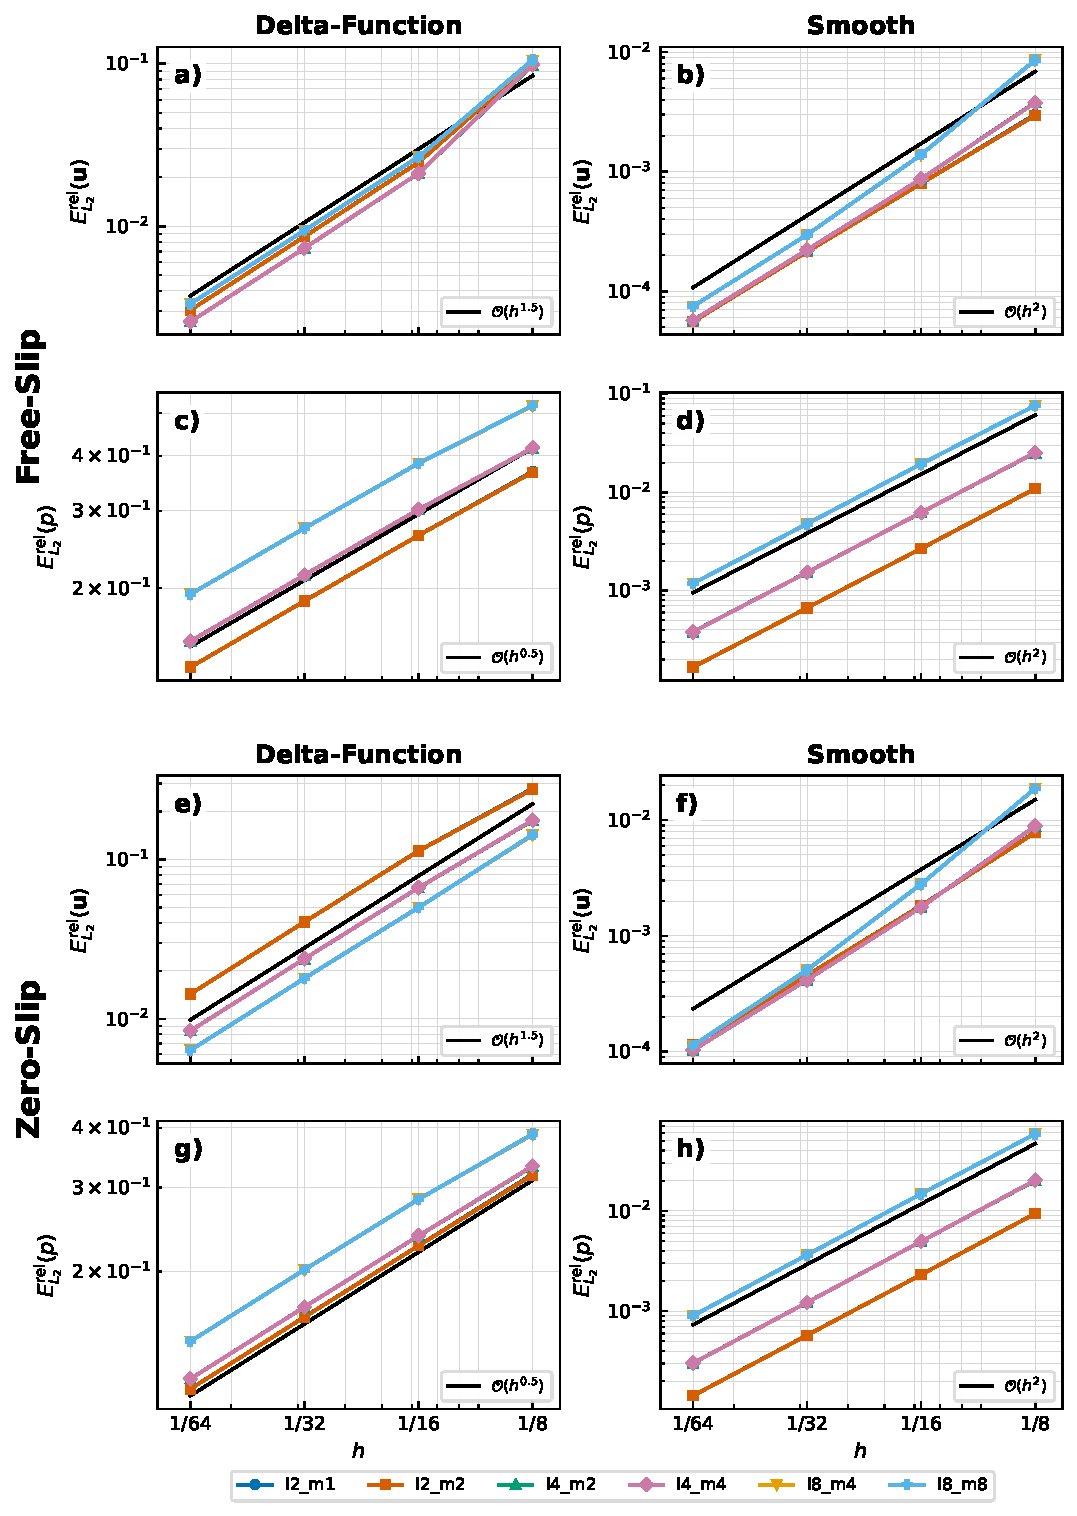
\includegraphics[width=0.98\linewidth]{figure_4_kramer_spherical_convergence.pdf}
    \caption{Velocity and pressure convergence for the four spherical Kramer cases.}
    \label{fig:kramer_velocity_pressure_convergence}
\end{figure}

The corresponding velocity and pressure error values and observed convergence
rates are provided in the split tables on the following pages. Each case is
reported in two tables, with three \((l,m,k)\) groups per table.

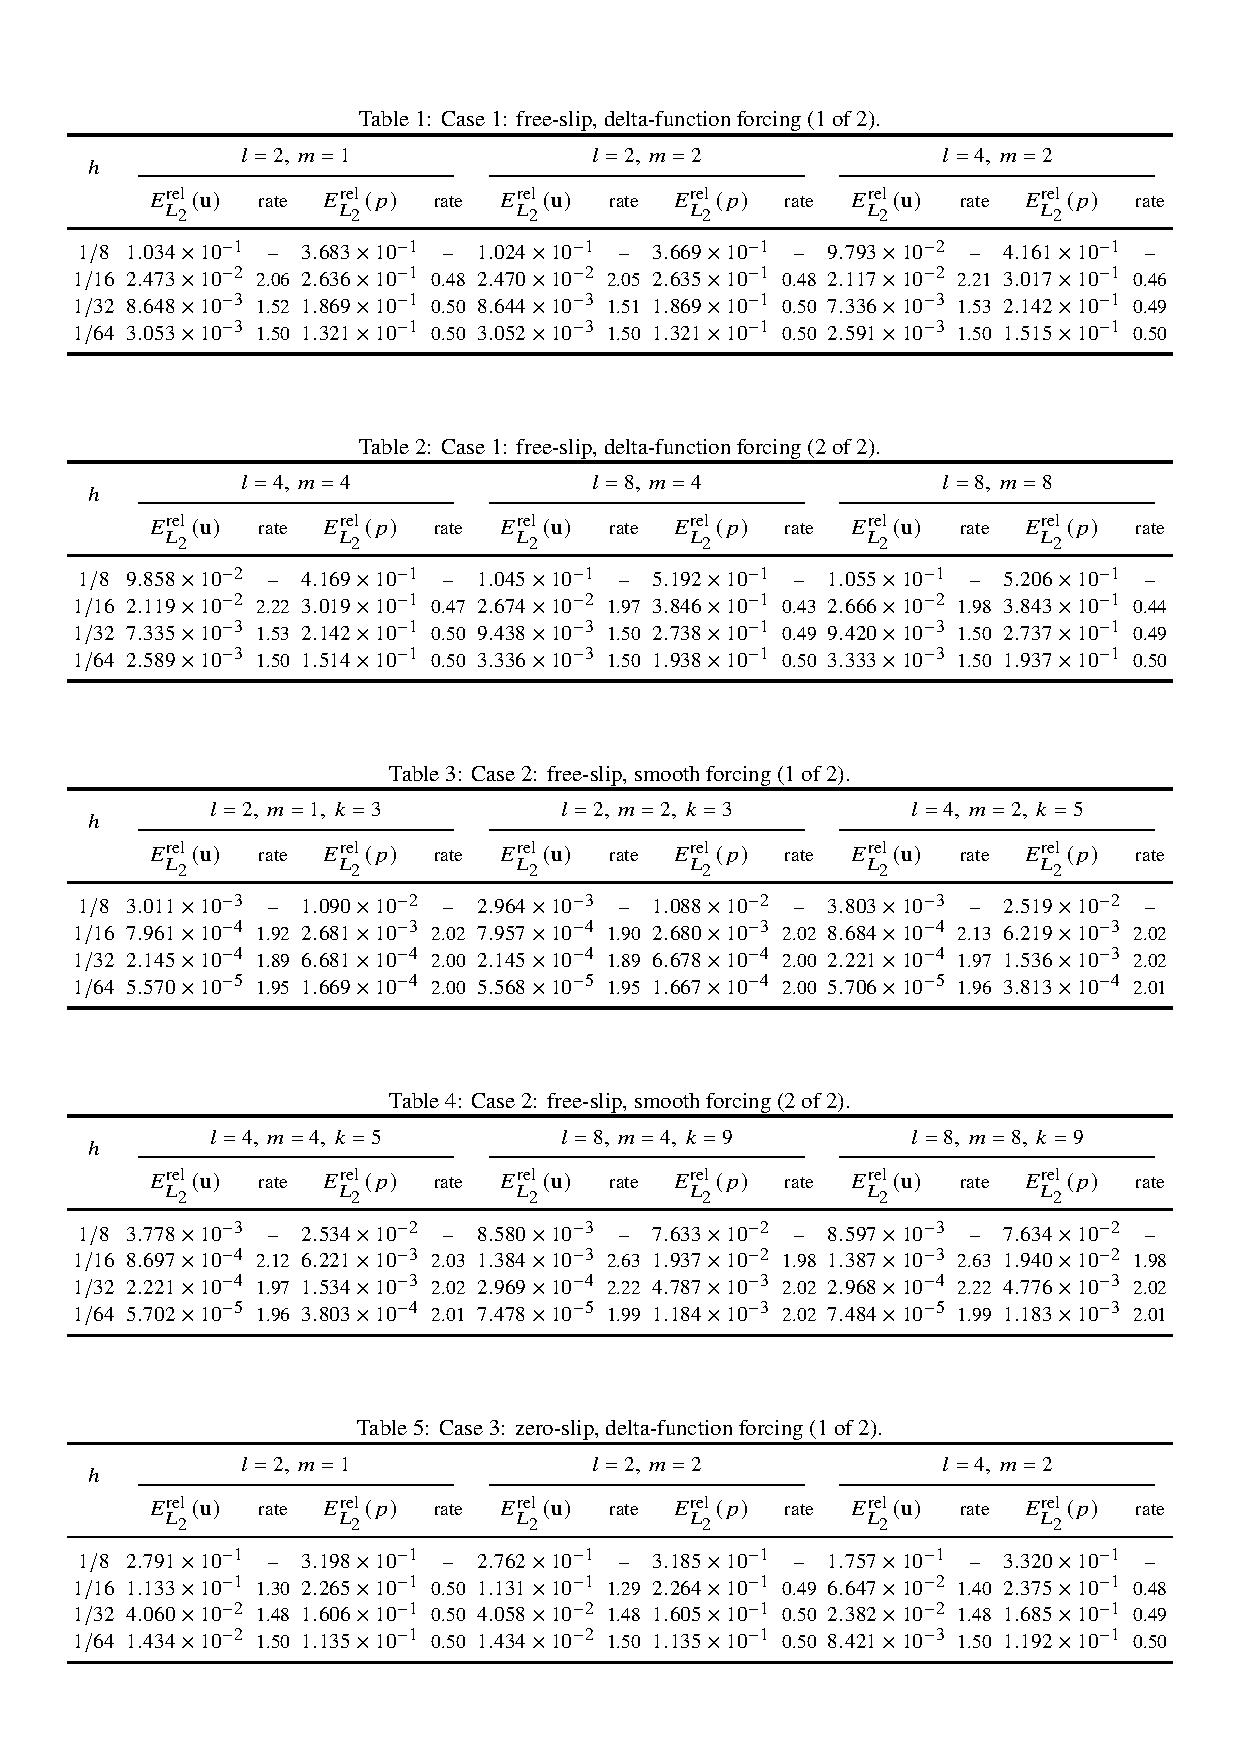
\includepdf[pages=-,fitpaper=true,pagecommand={\thispagestyle{plain}}]{table_figure_4_kramer_convergence.pdf}

\subsection{Boundary velocity and radial-stress convergence}

Boundary metrics are evaluated using relative \(L_2\) norms on the inner and outer spherical surfaces. The reported boundary table focuses on Case~1, the free-slip delta-function benchmark, because this is the most demanding configuration for boundary post-processing. Boundary velocity errors decrease rapidly on the coarse refinements, with rates near third to fourth order on the outer boundary. On the finest refinement the inner-boundary velocity rates reduce to approximately 2.3--2.6, while the outer boundary remains higher for the lower spherical harmonics. This difference is consistent with the boundary geometry and forcing distribution: the inner and outer surfaces have different radii, surface areas, analytical amplitudes, and interpolation errors, so their error constants are not expected to match.

Radial normal stress is a more sensitive diagnostic than velocity because it combines pressure with derivatives of the velocity field and is evaluated on curved boundaries. The UW3 stress errors converge systematically, but the observed rates are more variable than the volume velocity and pressure rates. Coarse-grid rates can be high because the calculation is still pre-asymptotic; the finest-grid radial-stress rates are closer to first-to-second order, with inner-boundary rates around 1.7--1.9 and outer-boundary rates depending more strongly on \((l,m,k)\). This behaviour is physically plausible for delta-function forcing because stress recovery is affected by the pressure singularity, derivative approximation, boundary quadrature, and the weak free-slip condition. The important result is therefore monotonic reduction and plausible asymptotic scaling, not equality of inner and outer boundary magnitudes.

\begin{figure}[H]
    \centering
    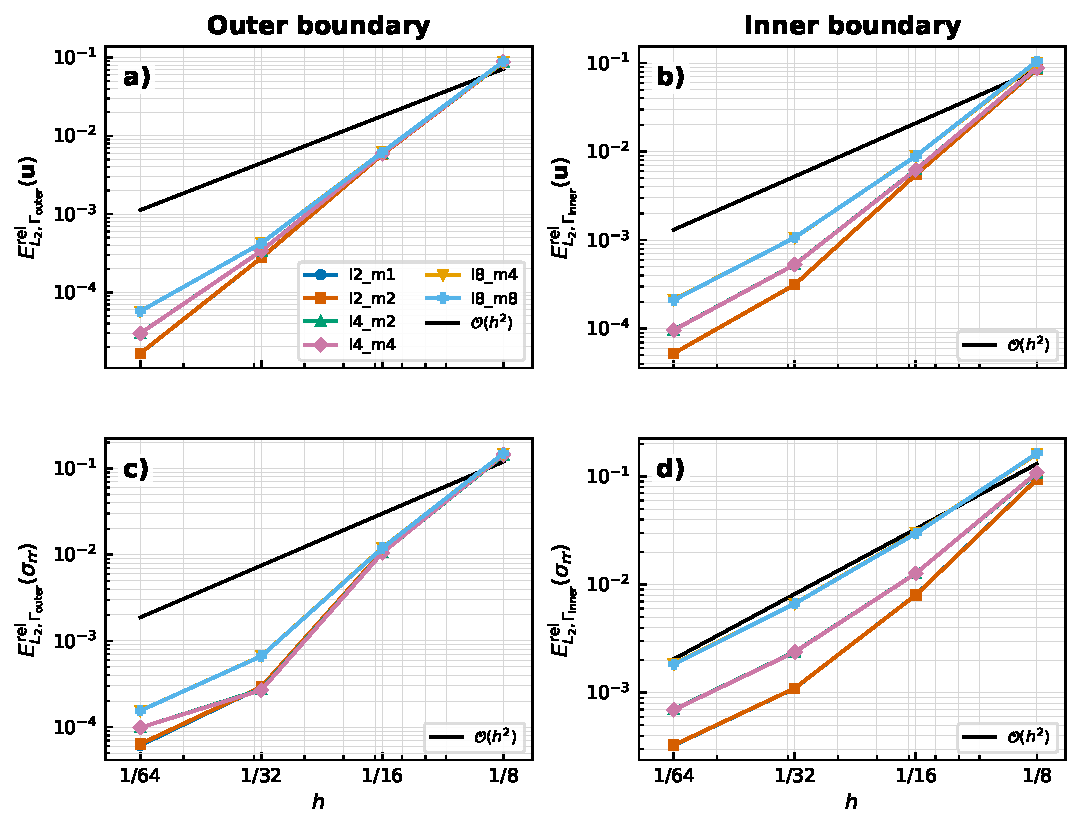
\includegraphics[width=0.98\linewidth]{figure_7_kramer_boundary_convergence.pdf}
    \caption{Boundary velocity and radial normal-stress convergence on the inner and outer spherical boundaries.}
    \label{fig:kramer_boundary_convergence}
\end{figure}

The boundary velocity and radial normal-stress error values are provided in the
split tables on the following pages, again using three \((l,m,k)\) groups per
table.

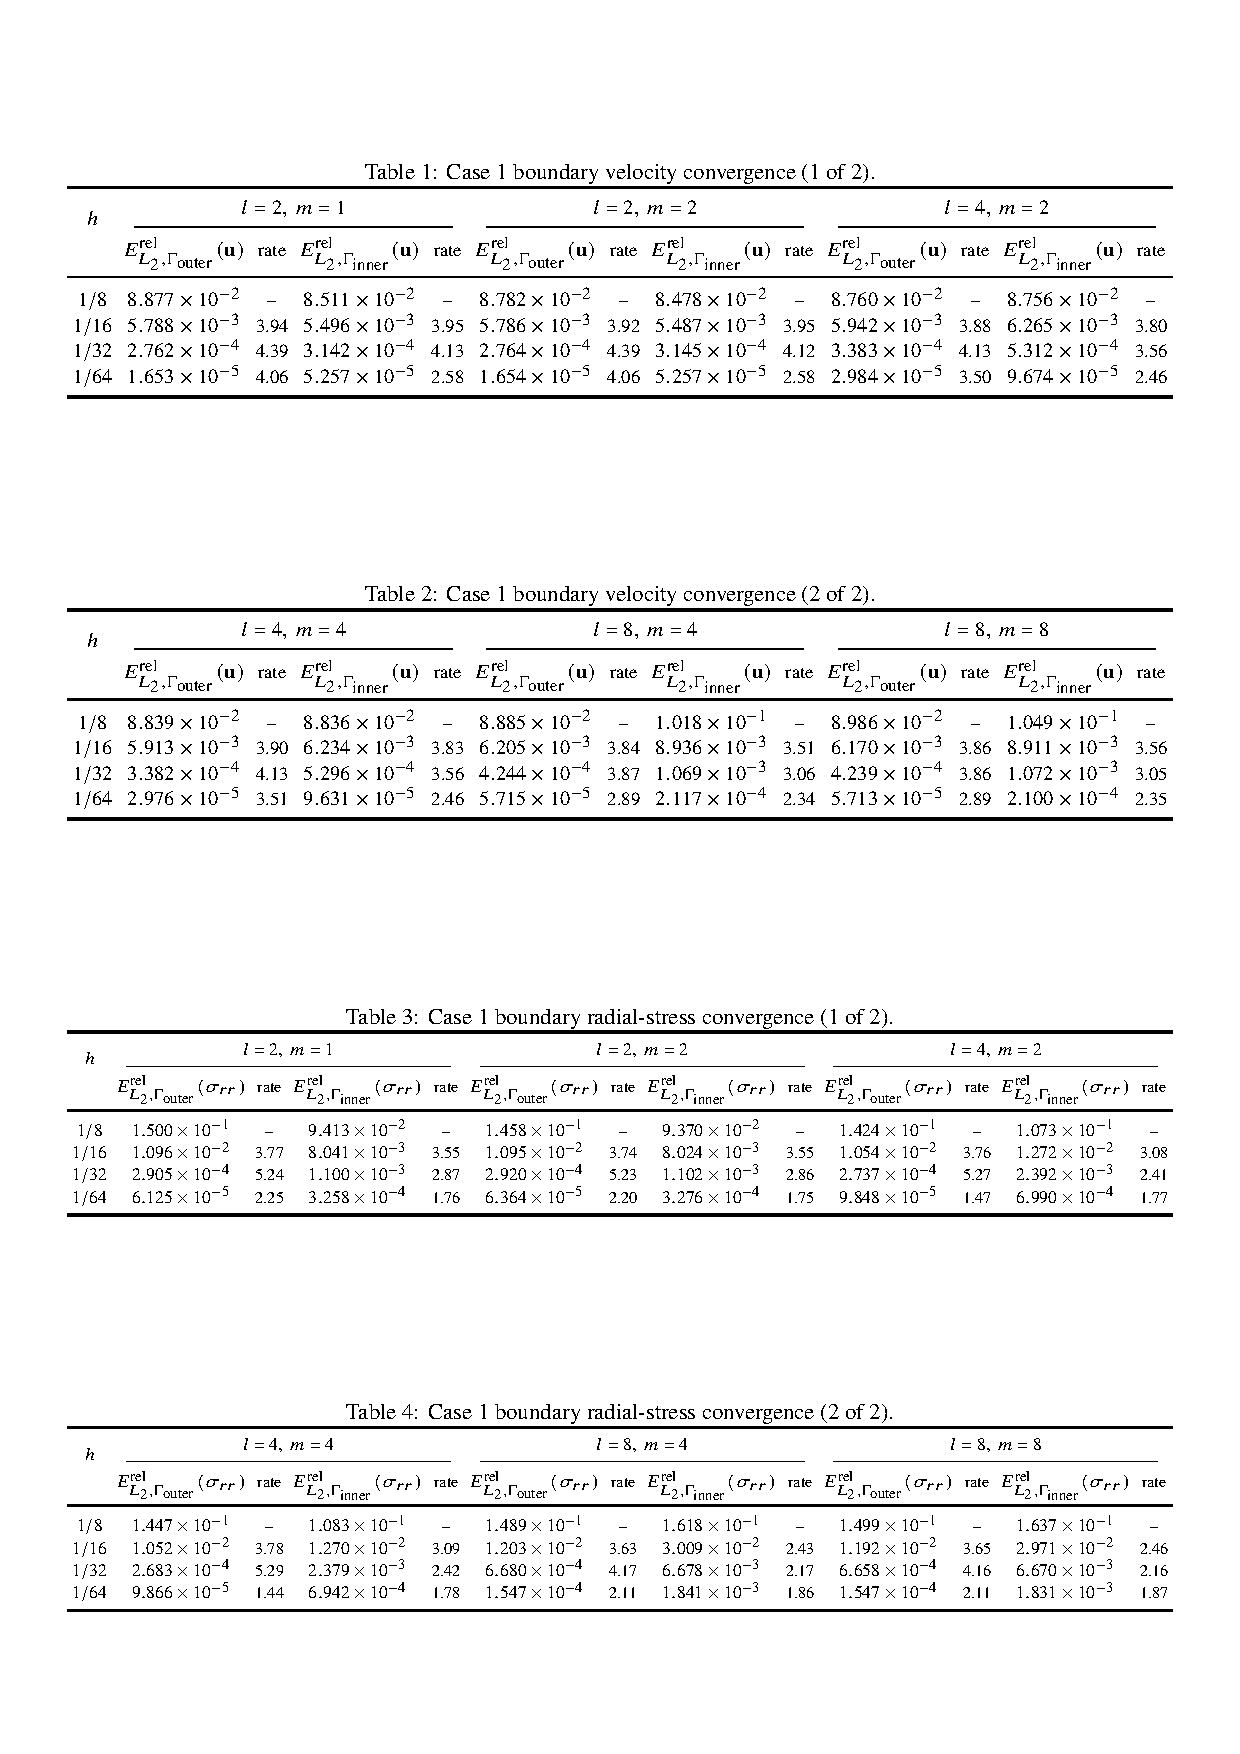
\includepdf[pages=-,fitpaper=true,pagecommand={\thispagestyle{plain}}]{table_figure_7_kramer_boundary_convergence.pdf}

\section{Discussion}

The UW3 results reproduce the key distinction between smooth and delta-function forcing, but the smooth velocity convergence is lower than the ideal third-order rate reported for the curved/isoparametric Fluidity calculations of \citet{kramer2021}. Instead, the observed smooth velocity rates are closer to second order, while the smooth pressure rates remain close to the expected second order. This separation is diagnostically useful: the Stokes solution and pressure approximation are behaving consistently, but the velocity field is not yet reaching the full curved-geometry asymptotic regime. A likely explanation is that geometry approximation, boundary representation, or the interaction between the spherical mesh and weak boundary conditions limits the velocity error before the polynomial interpolation error does.

The anomalous and suboptimal rates occur primarily in the delta-function cases and in boundary-derived stress quantities. These are the locations where theory predicts reduced regularity and where the numerical method must represent jumps or localised forcing. Continuous pressure further limits the delta pressure rate, while radial stress inherits both pressure error and velocity-gradient error. Higher \((l,m)\) values increase angular complexity, raising error constants and delaying asymptotic behaviour. Free-slip enforcement can also affect constants because tangential traction and normal-flow constraints must be represented accurately on a curved surface; penalty and Nitsche-style weak enforcement may therefore give different stress sensitivities even when the volume norms converge similarly.

\section{Comparison with previous benchmarks}

The UW3 pressure convergence and delta-forcing velocity trends are consistent with the Fluidity benchmark results of \citet{kramer2021}: smooth pressure is close to \(O(h^2)\), and delta cases show approximately \(O(h^{1.5})\) velocity and \(O(h^{0.5})\) pressure convergence. The main difference is the smooth-case velocity rate. Kramer et al. report third-order velocity convergence for smooth spherical cases with curved/isoparametric geometry, whereas the present UW3 results are closer to second order. This difference suggests that the current UW3 benchmark configuration is not yet realising the full asymptotic \(P_2\) velocity rate in curved spherical geometry. Differences in mesh generation, geometric order, boundary-condition enforcement, quadrature, solver tolerances, and pressure normalisation can all affect the observed constants and rates. The boundary pressure and stress diagnostics extend the comparison by testing post-processing quantities that are important for spherical geodynamics, including normal stress on curved shell boundaries.

\section{Summary and conclusions}

The Kramer spherical benchmark confirms that Underworld3 reproduces the main analytical Stokes benchmark trends for smooth and delta-function forcing in a spherical shell. Smooth pressure converges at the expected second-order rate, but smooth velocity convergence is closer to second order than to the ideal third-order \(P_2\) rate, indicating a likely geometric or boundary-representation limitation in the current setup. Delta-function cases exhibit the reduced rates predicted by the benchmark theory and observed by \citet{kramer2021}. Boundary pressure and radial normal-stress metrics converge systematically and provide additional verification of stress recovery and curved-boundary post-processing. Overall, the results support UW3 spherical Stokes verification while identifying smooth-case velocity convergence as the main item requiring further investigation.

\bibliographystyle{plainnat}
\bibliography{kramer_spherical_benchmark_report_refs}

\end{document}
